\documentclass{beamer}
\usepackage[T1]{fontenc}
\usepackage[utf8]{inputenc}
\usepackage{lmodern}
\usepackage[english]{babel}
\usepackage{tikz}
\usetheme{Warsaw}

\title[\textsc{Fabrication and measurements of NIS junctions}]{\textsc{Fabrication and measurements of\\NIS junctions to characterize\\plasma etching}}
\author{\textsc{Nicolas Paillet}}
\institute{Aalto University}
\date{11 August 2015}

\setbeamersize{text margin left=0.5cm,text margin right=0.5cm}

\begin{document}
\begin{frame}
    \titlepage
\end{frame}

    
    \begin{frame}
        \frametitle{\textsc{The nanowires project}}
        \framesubtitle{Introduction}
        Two types of InAs Nanowires coming from Copenhaguen : \\
        \begin{itemize}
            \item[$\bullet$]{Without barrier, and covered with Al}
            \item[$\bullet$]{With InGaAs barrier, without Al} 
        \end{itemize}
         
        For the covered ones :
        \begin{itemize}        
        \item[$\longrightarrow$] {Al heavily oxidized by the travel}
        \item[$\longrightarrow$] {Get rid of this oxide by Plasma Etching}
        \item[$\longrightarrow$] {Fabrication of NIS structures to characterize the Plasma}
        \end{itemize}
    \end{frame}

    \begin{frame}
        \frametitle{\textsc{The beginning}}
        \framesubtitle{Lack of rigour}
        
        First we made some tests that are not very relevant :
        \begin{itemize}
            \item [$\bullet$]{Two pad patterns $\Longrightarrow$ not handy for 4 probe measurements}
            \item [$\bullet$]{Measurements made with bounds with Matlab}
            \item[$\longrightarrow$]{Not efficient nor relevant}
        \end{itemize}
        
        \vspace{0.4cm}
        
        \indent$\Longrightarrow$ Need of a more systematic protocol
        
        \begin{itemize}
        \item[$\longrightarrow$]{Design of a new pattern}
        \item[$\longrightarrow$]{Measurements with a probestation}
        \end{itemize}
        
        \vspace{0.3cm}
        
        \centering
        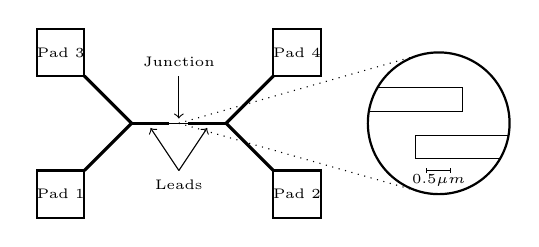
\begin{tikzpicture}[scale=0.6]
                    \draw [thick](0,0)--++(1,0)--++(0,1)--++(-1,0)--cycle;
                    \draw [thick](0,3)--++(1,0)--++(0,1)--++(-1,0)--cycle;
                    \draw [thick](5,0)--++(1,0)--++(0,1)--++(-1,0)--cycle;
                    \draw [thick](5,3)--++(1,0)--++(0,1)--++(-1,0)--cycle;
                    \draw [very thick](1,1)--(2,2);
                    \draw [very thick](1,3)--(2,2);
                    \draw [very thick](5,1)--(4,2);
                    \draw [very thick](5,3)--(4,2);
                    \draw [very thick](2,2)--(2.8,2);
                    \draw [very thick](4,2)--(3.2,2);
                    \draw (2.8,2)--(3.2,2);
                    \draw [->] (3,3)--(3,2.1);
                    \draw (3,3)node[above]{\tiny{Junction}};
                    \draw (0.5,0.5)node{\tiny{Pad 1}};
                    \draw (0.5,3.5) node{\tiny{Pad 3}};
                    \draw (5.5,0.5)node{\tiny{Pad 2}};
                    \draw (5.5,3.5)node{\tiny{Pad 4}};
                    \draw [->] (3,1)--(2.4,1.9);
                    \draw [->] (3,1)--(3.6,1.9);
                    \draw (3,1)node[below]{\tiny{Leads}};
                    \draw [dotted,thin] (3,2)--(8.1,3.45);
                    \draw [dotted,thin] (3,2)--(8.1,0.55);
                    \draw [thick](8.5,2) circle(1.5);
                    \draw (7.2,2.75)--(9,2.75)--(9,2.25)--(7.02,2.25);
                    \draw (9.8,1.25)--(8,1.25)--(8,1.75)--(9.98,1.75);
                    \draw (8.25,1.05)--(8.25,0.95);
                    \draw (8.75,1.05)--(8.75,0.95);
                    \draw (8.25,1)--(8.75,1);
                    \draw (8.5,0.8)node{\tiny{0.5$\mu m$}};

                \end{tikzpicture}
                
    \end{frame}

    \begin{frame}[allowframebreaks]
        \frametitle{\textsc{Reference samples}}
        \framesubtitle{Room temperature measurements}
            $\bullet$  Clean Contact Al + Cu
            \vspace{0.3cm}
            
            \begin{center}
            \includegraphics[width=280pt]{Rclean.png}
            \[R=\sum_{Cu,Al}\dfrac{\rho l}{S}\simeq 78 \Omega\]
            \end{center}
            
            $\bullet$  Strong Oxidation reference 10min / 200mbar
            \vspace{0.5cm}
            
            \includegraphics[width=330pt]{ConductanceFitStrongOx.png}
             \vspace{1cm}
             
            $\bullet$  Regular Oxidation Reference 2min / 2mbar
            \vspace{0.5cm}
            
            \includegraphics[width=330pt]{ConductanceFitOx.png}
    \end{frame}
    
    \begin{frame}[allowframebreaks]
        \frametitle{\textsc{Plasma Tests}}
        \framesubtitle{Room temperature measurements}
        $\bullet$  Time of Plasma
        \vspace{0.5cm}
        
        \includegraphics[width=330pt]{R_Time.png}
        \vspace{1cm}
        
        $\bullet$  Position of the sample
        \vspace{0.5cm}
        
        \includegraphics[width=330pt]{R_Position.png}

    \end{frame}
    
    \begin{frame}[allowframebreaks]
        \frametitle{\textsc{Before the LISA maintenance}}
        \framesubtitle{Low temperature measurements}

        $\bullet$ Regular Oxidation 2min / 2mbar NIS
        \vspace{0.3cm}
        
        \includegraphics[width=330pt]{BeforeLISAOx.png}
%         \vspace{1cm}
%         
%         $\bullet$ Strong Oxidation 10min / 200mbar NIS
%         \vspace{0.5cm}
%         
%         \includegraphics[width=330pt]{}
%         \vspace{1cm}
        
%         $\bullet$ Temperature Sweep
%         \vspace{0.5cm}
        
%         \includegraphics[width=330pt]{}
        
        
    \end{frame}
    
    \begin{frame}[allowframebreaks]
        \frametitle{\textsc{After LISA maintenance}}
        \framesubtitle{Low temperature measurements}
        $\bullet$  Regular Oxidation just after the maintenance
        \vspace{0.3cm}
        
        \includegraphics[width=330pt]{AfterLISAOx.png}
        \vspace{1cm}
                       
        $\bullet$  Burned Samples with 10 min of plasma
        \vspace{0.5cm}
        
       \includegraphics[width=165pt]{Burned2.png}
       \includegraphics[width=165pt]{Burned1.png}
              
              \vspace{3cm}
              
       $\bullet$ Wafer etching : 10 min of plasma is too much
       \vspace{0.5cm}
       
       \includegraphics[width=165pt]{tilt1.png}
       \includegraphics[width=165pt]{tilt2.png}
        \vspace{3cm}
        
        $\bullet$ Plasma Oxidation
        \vspace{0.3cm}
        
        \includegraphics[width=330pt]{PlasmaOx.png}
        \vspace{1cm}
        
        $\bullet$ Regular Oxidation reference for previous sample
        
        \centering
        \includegraphics[width=330pt]{RegularOxRef.png}
        \vspace{1cm}

    \end{frame}
    
    \begin{frame}
        \frametitle{\textsc{Conclusion}}
        \begin{LARGE}
        \centering    
        Thank you for your attention !
        \vspace{0.5cm}
        
        \centering
        If you have any questions please ask.
        
        \end{LARGE}

       \end{frame}
       
    \end{document}
